\documentclass[11pt,twoside,a4paper]{article}
% http://www-h.eng.cam.ac.uk/help/tpl/textprocessing/latex_maths+pix/node6.html symboles de math
% http://fr.wikibooks.org/wiki/Programmation_LaTeX Programmation latex (wikibook)
%=========================== En-Tete =================================
%--- Insertion de paquetages (optionnel) ---
\usepackage[english]{babel}
\usepackage{a4}	             % pour la taille   
\usepackage[T1]{fontenc}     % pour les font postscript
\usepackage{epsfig}          % pour gerer les images
%\usepackage{psfig}
\usepackage{amsmath, amsthm} % tres bon mode mathematique
\usepackage{amsfonts,amssymb}% permet la definition des ensembles
\usepackage{float}           % pour le placement des figure
\usepackage{verbatim}
\usepackage{longtable} % pour les tableaux de plusieurs pages
\usepackage[table]{xcolor} % couleur de fond des cellules de tableaux
\usepackage{lastpage}

% \usepackage[top=1.5cm, bottom=1.5cm, left=1.5cm, right=1.5cm]{geometry}
% gauche, haut, droite, bas, entete, ente2txt, pied, txt2pied
\usepackage{vmargin}
\setmarginsrb{1.0cm}{1.0cm}{1.0cm}{1.0cm}{15pt}{3pt}{60pt}{25pt}

\usepackage{lscape} % changement orientation page
%\usepackage{frbib} % enlever pour obtenir references en anglais
% --- style de page (pour les en-tete) ---
\pagestyle{headings}

\def\MainTitle{The ship and it's ecology}

% % % en-tete et pieds de page configurables : fancyhdr.sty

% http://www.trustonme.net/didactels/250.html

% http://ww3.ac-poitiers.fr/math/tex/pratique/entete/entete.htm
% http://www.ctan.org/tex-archive/macros/latex/contrib/fancyhdr/fancyhdr.pdf
\usepackage{fancyhdr}
\pagestyle{fancy}
% \newcommand{\chaptermark}[1]{\markboth{#1}{}}
% \newcommand{\sectionmark}[1]{\markright{\thesection\ #1}}
\fancyhf{}
\fancyhead[LE,RO]{\bfseries\thepage}
\fancyhead[LO]{\bfseries\rightmark}
\fancyhead[RE]{\bfseries\leftmark}
\fancyfoot[LE]{\thepage /\pageref{LastPage} \hfill
	\MainTitle 
\hfill 
\includegraphics[width=0.5cm]{img/logo_glider.png} }
\fancyfoot[RO]{
\includegraphics[width=0.5cm]{img/logo_glider.png} \hfill
	\MainTitle 
\hfill \thepage /\pageref{LastPage}}
\renewcommand{\headrulewidth}{0.25pt}
\renewcommand{\footrulewidth}{0.50pt}
\addtolength{\headheight}{0.5pt}
\fancypagestyle{plain}{
	\fancyhead{}
	\renewcommand{\headrulewidth}{0pt}
}

%--- Definitions de nouvelles commandes ---
\newcommand{\N}{\mathbb{N}} % les entiers naturels

%--- Definitions de nouvelles couleurs ---
\definecolor{verylightgrey}{rgb}{0.8,0.8,0.8}
\definecolor{verylightgray}{gray}{0.80}
\definecolor{lightgrey}{rgb}{0.6,0.6,0.6}
\definecolor{lightgray}{gray}{0.6}

%============================= Corps =================================
\begin{document}

\setlength\parindent{0pt}



%% ~\\
%% \vfill

\begin{center} 
\includegraphics[width=0.75\textwidth]{img/acw_logo8.jpg} \end{center}

\begin{center}
	\textbf{\Large \MainTitle }~\\
	%% \textbf{or}~\\
	%% \textbf{\large The ship and it's ecology}~\\
\end{center}

\tableofcontents

\vfill

%% ~\\

%% \clearpage

Did you wonder how many creatures are inhabitating the Ship and what's their name? That's why I put up a list for you with their common names but also with the latin names! I didn't invent them, but the developers at Creatureslabs did. Some of them are really funny, you'll smile, for sure! I added to each creature where it usually lives and what it needs for it's living. There is a real food chain existing in all of the four terrariums, a constant"Eat and get eaten". ~\\

\begin{tabular}[h]{ p{1.60cm} p{0.95cm} p{2.55cm} p{12.00cm} }
	\rowcolor[gray]{0.50}	\textbf{Creature}					&	\textbf{Name}	&	\textbf{Latin Name}			&	\textbf{Located}		\\ 
																&					&								&							\\ 
	\begin{minipage}[ht]{1.55cm} 
\includegraphics[width=1.50cm]{img/bhead.jpg} \end{minipage}		
																&	Norn			&	Cyberlifogenis cutis		&	Everywhere on the ship, but prefers the Norn-Terrarium.	\\
	\begin{minipage}[ht]{1.55cm} 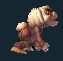
\includegraphics[width=1.50cm]{img/ettin1.jpg} \end{minipage}		
																&	Ettin			&	Cyberlifogenis kleptomania	&	To be found everywhere on the ship, doesn't absolutely need to be in it's home terrarium (the desert) but likes to return there, especially after having found portable equipment...	\\
	\begin{minipage}[ht]{1.55cm} 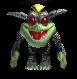
\includegraphics[width=1.50cm]{img/bert.jpg} \end{minipage}		
																&	Grendel			&	Cyberlifogenis vicious		&	Found everywhere on the ship. It's home terrarium is the jungle.	\\ 
\end{tabular} ~\\

\vfill

\clearpage

\section*{
\includegraphics[width=1.50cm]{img/nornt.jpg} Norn Terrarium\markboth{Norn Terrarium}{Norn Terrarium}}
\addcontentsline{toc}{section}{Norn Terrarium}

\begin{longtable}{ p{1.60cm} p{1.95cm} p{2.55cm} p{11.00cm} }
	\rowcolor[gray]{0.50}	\textbf{Creature}					&	\textbf{Name}	&	\textbf{Latin Name}			&	\textbf{Located}		\\ 
	\endfirsthead
	\rowcolor[gray]{0.80} \multicolumn{4}{ c }{\emph{Continued from previous page}}				\\
	\rowcolor[gray]{0.75}	\textbf{Creature}					&	\textbf{Name}	&	\textbf{Latin Name}			&	\textbf{Located}		\\
	\endhead
	\rowcolor[gray]{0.80} \multicolumn{4}{ c }{\emph{Continued on next page}}					\\
	\endfoot
	\hline
	\endlastfoot
																&					&								&							\\ 
	\begin{minipage}[ht]{1.55cm} 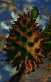
\includegraphics[width=1.50cm]{img/spikel2.jpg} \end{minipage}		
																&	Pumperspikel	&	Pumpica spikelum		
																&	Meant is the Pumperspikel tree where theses fruits grow. The seeds are a very good food source for norns.	\\
	\begin{minipage}[ht]{1.55cm} 
\includegraphics[width=1.50cm]{img/apfel.jpg} \end{minipage}		
																&	Apple			&	Malus albia		
																&	Apples grow on the apple tree. (how smart! :-))	\\
	\begin{minipage}[ht]{1.55cm} 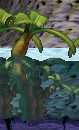
\includegraphics[width=1.50cm]{img/watplant.jpg} \end{minipage}		
																&	Waterplant		&	Yucca \newline aquatiform		
																&	There are three of these waterplants located in the pond. They don't die out.	\\
	\begin{minipage}[ht]{1.55cm} 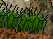
\includegraphics[width=1.50cm]{img/grass.jpg} \end{minipage}		
																&	Grass 			&	Poa verdanata		
																&	Needs warmth, humidity and light for growing. 	\\
	\begin{minipage}[ht]{1.55cm} 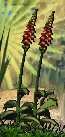
\includegraphics[width=1.50cm]{img/fox.jpg} \end{minipage}		
																&	Foxglove		&	Digitalis \newline bensimpsus		
																&	Needs warmth, humidity and light to grow. Can die out if there are too less seeds disseminated. You can bring it back by means of the seed bank. It's nectar is food for bees and butterflies which pollinate the foxgloves in return.	\\
	\begin{minipage}[ht]{1.55cm} 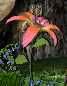
\includegraphics[width=1.50cm]{img/pinkplant.jpg} \end{minipage}		
																&	Pinky Plant		&	Dianthus \newline statiphytes		
																&	This plant doesn't die out. Food plant for bees and butterflies.	\\
	\begin{minipage}[ht]{1.55cm} 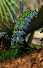
\includegraphics[width=1.50cm]{img/blaupfl.jpg} \end{minipage}		
																&	Blue Flower		&	Cynoflora \newline morrisii		
																&	This plant doesn't die out. Food plant for bees, butterflies and kolibris.	\\
	\begin{minipage}[ht]{1.55cm} 
\includegraphics[width=1.50cm]{img/grazer.jpg} \end{minipage}		
																&	Grazer			&	Scatus \newline harmenius		
																&	Peaceful, eats grass (therefore it's name!).	\\
	\begin{minipage}[ht]{1.55cm} 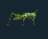
\includegraphics[width=1.50cm]{img/heug.jpg} \end{minipage}		
																&	Grasshopper		&	Idealus \newline roberticum		
																&	Eats leaves and hoppes from here to there...	\\
	\begin{minipage}[ht]{1.55cm} 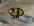
\includegraphics[width=1.50cm]{img/bien.jpg} \end{minipage}		
																&	Bee				&	Bombillius lisasillius		
																&	Needs nectar from the flowers of plants, lives in bee hives. Be carful! it stings your norns when they try to play with them! "Ouch!"	\\
	\begin{minipage}[ht]{1.55cm} 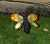
\includegraphics[width=1.50cm]{img/schmet.jpg} \end{minipage}		
																&	Butterfly		&	Papillio \newline haywardian		
																&	The caterpillars eats leaves, then they will climb the plants and transform into beautiful butterflies which need the flowers of the plants resp. it's nectar as food.	\\
	\begin{minipage}[ht]{1.55cm} 
\includegraphics[width=1.50cm]{img/ameise.jpg} \end{minipage}		
																&	Ant				&	Formica \newline saunterous \newline albia		
																&	Takes care of the organic deposits and detritus	\\
	\begin{minipage}[ht]{1.55cm} 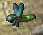
\includegraphics[width=1.50cm]{img/libelle.jpg} \end{minipage}		
																&	Dragonfly		&	Flitus \newline bhomicus		
																&	Eats other insects, the larvae eat the leaves of the water plant, so dragonflies need water around to lay there eggs in.	\\
	\begin{minipage}[ht]{1.55cm} 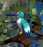
\includegraphics[width=1.50cm]{img/kolibri.jpg} \end{minipage}		
																&	Hummingbird		&	Tristaniana bussia		
																&	Needs nectar of flowers to survive. 	\\
	\begin{minipage}[ht]{1.55cm} 
\includegraphics[width=1.50cm]{img/taube.jpg} \end{minipage}		
																&	Wood Pigeon		&	Columba \newline cantellia		
																&	Eats different insects, fruits, seeds. 	\\
	\begin{minipage}[ht]{1.55cm} 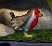
\includegraphics[width=1.50cm]{img/robin.jpg} \end{minipage}		
																&	Robin			&	Charltonian \newline albia		
																&	Eats insects and makes it's nest sometimes in the apple tree where you can see (with a little luck!) the young robings getting old enough to fly off.	\\
	\begin{minipage}[ht]{1.55cm} 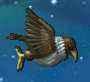
\includegraphics[width=1.50cm]{img/hawk.jpg} \end{minipage}		
																&	Gosh Hawk		&	Assipter \newline stewardian		
																&	Eats grazers.	\\
	\begin{minipage}[ht]{1.55cm} 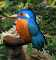
\includegraphics[width=1.50cm]{img/king.jpg} \end{minipage}		
																&	Kingfisher		&	Alcedo makious cristoph		
																&	Catches and eats the stickletrout, that's why you can find the kingfisher always near the pond. 	\\
	\begin{minipage}[ht]{1.55cm} 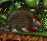
\includegraphics[width=1.50cm]{img/igel.jpg} \end{minipage}		
																&	Hedgehog		&	Erinaceus albia		
																&	Eats insects and snails.	\\
	\begin{minipage}[ht]{1.55cm} 
\includegraphics[width=1.50cm]{img/hoppity2.jpg} \end{minipage}		
																&	Hoppity			&	Hoppis napes roo		
																&	Eats fruits. Can multiply extremly fast if food situation allows and your game can ge flooded with hoppities...	\\
	\begin{minipage}[ht]{1.55cm} 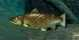
\includegraphics[width=1.50cm]{img/stichling.jpg} \end{minipage}		
																&	Stickletrout	&	Salar stikus		
																&	Lives in the pond and eats (almost) anyyting what's falling into the water, above all insects.	\\
	\begin{minipage}[ht]{1.55cm} 
\includegraphics[width=1.50cm]{img/schnecke.jpg} \end{minipage}		
																&	Snail			&	Barrus \newline osullivus		
																&	Eats organic detritus. 	\\
\end{longtable} %% ~\\

\clearpage

\section*{
\includegraphics[width=1.50cm]{img/wuestt.jpg} Desert Terrarium\markboth{Desert Terrarium}{Desert Terrarium}}
\addcontentsline{toc}{section}{Desert Terrarium}

\begin{tabular}[h]{ p{1.60cm} p{1.95cm} p{2.55cm} p{11.00cm} }
	\rowcolor[gray]{0.50}	\textbf{Creature}					&	\textbf{Name}	&	\textbf{Latin Name}			&	\textbf{Located}		\\ 
																&					&								&							\\ 
	\begin{minipage}[ht]{1.55cm} 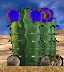
\includegraphics[width=1.50cm]{img/cacbana.jpg} \end{minipage}		
																&	Cacbana			&	Burbania \newline barnabicia		
																&	Needs lot of light and heat, it's more succulent.	\\
	\begin{minipage}[ht]{1.55cm} 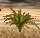
\includegraphics[width=1.50cm]{img/wgrass.jpg} \end{minipage}		
																&	Desert Grass	&	Festuca \newline xerophilus		
																&	Adapted to the desert, needs light and heat.	\\
	\begin{minipage}[ht]{1.55cm} 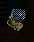
\includegraphics[width=1.50cm]{img/balloon.jpg} \end{minipage}		
																&	Balloon Bug		&	Apterus \newline claudinio		
																&	Lives with and from the Cacbanas.	\\
	\begin{minipage}[ht]{1.55cm} 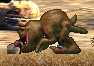
\includegraphics[width=1.50cm]{img/gnarler.jpg} \end{minipage}		
																&	Gnarler			&	Hungarius \newline oscari		
																&	Eats the stones from the vulcano once they're cooled. Strange diet, but make sure there are enough stones laying around so the Gnarlers won't die out.	\\
	\begin{minipage}[ht]{1.55cm} 
\includegraphics[width=1.50cm]{img/meek.jpg} \end{minipage}		
																&	Meerk			&	Sciurus \newline harmanii		
																&	Eats Balloon Bugs and and likes to dig into the ground.	\\
	\begin{minipage}[ht]{1.55cm} 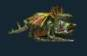
\includegraphics[width=1.50cm]{img/uglee.jpg} \end{minipage}		
																&	Uglee			&	Grendomorphis vulgaris		
																&	Eats Gnarler eggs which it spies during its flights.	\\
\end{tabular} ~\\

\clearpage

\section*{
\includegraphics[width=1.50cm]{img/junglet.jpg} Jungle Terrarium\markboth{Jungle Terrarium}{Jungle Terrarium}}
\addcontentsline{toc}{section}{Jungle Terrarium}

\begin{longtable}{ p{1.60cm} p{1.95cm} p{2.55cm} p{11.00cm} }
	\rowcolor[gray]{0.50}	\textbf{Creature}					&	\textbf{Name}	&	\textbf{Latin Name}			&	\textbf{Located}		\\ 
	\endfirsthead
	\rowcolor[gray]{0.80} \multicolumn{4}{ c }{\emph{Continued from previous page}}				\\
	\rowcolor[gray]{0.75}	\textbf{Creature}					&	\textbf{Name}	&	\textbf{Latin Name}			&	\textbf{Located}		\\
	\endhead
	\rowcolor[gray]{0.80} \multicolumn{4}{ c }{\emph{Continued on next page}}					\\
	\endfoot
	\hline
	\endlastfoot
																&					&								&							\\ 
	\begin{minipage}[ht]{1.55cm} 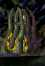
\includegraphics[width=1.50cm]{img/tendril.jpg} \end{minipage}		
																&	Tendril			&	Coeloformis \newline albia		
																&	Easy to grow, needs only a bit of humidity. Can even grow in complete darkness!	\\
	\begin{minipage}[ht]{1.55cm} 
\includegraphics[width=1.50cm]{img/pilz.jpg} \end{minipage}		
																&	Fungi			&	Amanita albia		
																&	Needs humidity, but can grow almost everywhere, also on darkness.	\\
	\begin{minipage}[ht]{1.55cm} 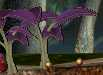
\includegraphics[width=1.50cm]{img/purbana.jpg} \end{minipage}		
																&	Purbana			&	Coleus \newline purpureum		
																&	This plant never dies out. Apart of this it doesn't play further role in the ecosystem....	\\
	\begin{minipage}[ht]{1.55cm} 
\includegraphics[width=1.50cm]{img/wespe.jpg} \end{minipage}		
																&	Wasp			&	Netelia davidum		
																&	Eats fruits and stings when getting annoyed!	\\
	\begin{minipage}[ht]{1.55cm} 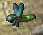
\includegraphics[width=1.50cm]{img/libelle.jpg} \end{minipage}		
																&	Dragonfly		&	Flitus \newline bhomicus		
																&	Eats other insects, the larvae eat the leaves of the water plant, so dragonflies need water around to lay there eggs in.	\\
	\begin{minipage}[ht]{1.55cm} 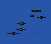
\includegraphics[width=1.50cm]{img/gnats.jpg} \end{minipage}		
																&	Gnats			&	Strawcium \newline gigantus		
																&	Only being seen in swarm. They eat male Grendels! Never seen until now? Yes, of course the do exist, watch closer and then you might be able to catch a glimps of them hovering between the leaves...	\\
	\begin{minipage}[ht]{1.55cm} 
\includegraphics[width=1.50cm]{img/lice.jpg} \end{minipage}		
																&	Rocklice		&	Jonti \newline praticilium		
																&	Eats insects, drills itself into the ground and get's nasty sometimes.	\\
	\begin{minipage}[ht]{1.55cm} 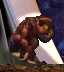
\includegraphics[width=1.50cm]{img/kobold.jpg} \end{minipage}		
																&	Kobold			&	Baldium \newline mysterious		
																&	Eats insects, fruits and other food which is brought into the jungle by other creatures. The Kobold is constantly a bit ill-tempered.	\\
	\begin{minipage}[ht]{1.55cm} 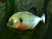
\includegraphics[width=1.50cm]{img/piranha2.jpg} \end{minipage}		
																&	Piranha			&	Viscious \newline fiscious		
																&	Dangerous! Eats every creature that falls into it's pond and there will be nothing left but a few bones...	\\
	\begin{minipage}[ht]{1.55cm} 
\includegraphics[width=1.50cm]{img/mossie.jpg} \end{minipage}		
																&	Mosquito		&	Mossee \newline darmicus		
																&	Ouch! Stings and very nasty!	\\
	\begin{minipage}[ht]{1.55cm} 
\includegraphics[width=1.50cm]{img/beetle.jpg} \end{minipage}		
																&	Rhino~Beetle	&	Tuffus \newline burchiium maximus		
																&	Eats organic detritus.\\
	\begin{minipage}[ht]{1.55cm} 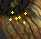
\includegraphics[width=1.50cm]{img/baks.jpg} \end{minipage}		
																&	Bacteria		&	Bhowmicoccus nornovora		
																&	Responsible for any kinds of infectuous illnesses in Norns! Cannot be seen by the naked eye, you need special tools to make them visible.	\\
\end{longtable} ~\\

\clearpage

\section*{
\includegraphics[width=1.50cm]{img/aquat.jpg} Aquarium\markboth{Aquarium}{Aquarium}}
\addcontentsline{toc}{section}{Aquarium}

\begin{longtable}{ p{1.60cm} p{1.95cm} p{2.55cm} p{11.00cm} }
	\rowcolor[gray]{0.50}	\textbf{Creature}					&	\textbf{Name}	&	\textbf{Latin Name}			&	\textbf{Located}		\\ 
	\endfirsthead
	\rowcolor[gray]{0.80} \multicolumn{4}{ c }{\emph{Continued from previous page}}				\\
	\rowcolor[gray]{0.75}	\textbf{Creature}					&	\textbf{Name}	&	\textbf{Latin Name}			&	\textbf{Located}		\\
	\endhead
	\rowcolor[gray]{0.80} \multicolumn{4}{ c }{\emph{Continued on next page}}					\\
	\endfoot
	\hline
	\endlastfoot
																&					&								&							\\ 
	\begin{minipage}[ht]{1.55cm} \includegraphics[width=1.00cm]{img/opalsch.jpg} \end{minipage}		
																&	Opal Sponge		&	Porifera opalite		
																&	Lives only in salt water.	\\
	\begin{minipage}[ht]{1.55cm} \includegraphics[width=1.00cm]{img/oschwam.jpg} \end{minipage}		
																&	Orange Sponge	&	Porifera \newline orangeboom		
																&	Lives only in salt water.	\\
	\begin{minipage}[ht]{1.55cm} \includegraphics[width=1.00cm]{img/seagrass.jpg} \end{minipage}		
																&	Gumin Grass		&	Poa guminum		
																&	Lives only in salt water. Can only grow if there's no other Gumin Grass or Orange Sponge growing nearby.	\\
	\begin{minipage}[ht]{1.55cm} \includegraphics[width=1.50cm]{img/mites.jpg} \end{minipage}		
																&	Aquamites		&	Aquatophagoides albia		
																&	They filter nutrients out of the water.	\\
	\begin{minipage}[ht]{1.55cm} \includegraphics[width=1.50cm]{img/wyst.jpg} \end{minipage}		
																&	Wyst			&	Cluelesseus \newline officiusous		
																&	They filter nutrients out of the water.	\\
	\begin{minipage}[ht]{1.55cm} \includegraphics[width=1.50cm]{img/handlef.jpg} \end{minipage}		
																&	Angel Fish		&	Gillium gillium		
																&	Eats the seeds of the Orange Sponge as well as those of the Opal Sponge and Gumin Grass and eats Wysts too	\\
	\begin{minipage}[ht]{1.55cm} \includegraphics[width=1.50cm]{img/clownf.jpg} \end{minipage}		
																&	Clown Fish		&	Premnas \newline hilariousis		
																&	Eats wysts and seeds of the Opal Sponge, of the Orange Sponge and of Gumin Grass.	\\
	\begin{minipage}[ht]{1.55cm} \includegraphics[width=1.50cm]{img/angelf.jpg} \end{minipage}		
																&	Handlefish		&	Ficious \newline tobiniuos \newline aquatonicus		
																&	Eats the seeds of the Orange Sponge as well as those of the Opal Sponge and Gumin Grass and eats Wysts too	\\
	\begin{minipage}[ht]{1.55cm} \includegraphics[width=1.50cm]{img/neonf.jpg} \end{minipage}		
																&	Neon Fish		&	Hyphessobrycon creaturelabiani		
																&	Eats the seeds of the Orange Sponge as well as those of the Opal Sponge and Gumin Grass and eats Wysts too	\\
	\begin{minipage}[ht]{1.55cm} \includegraphics[width=1.50cm]{img/tintf.jpg} \end{minipage}		
																&	Cuttlefish		&	Sushi \newline hazardous		
																&	Eats Wysts and shows colour change when annoyed.	\\
	\begin{minipage}[ht]{1.55cm} \includegraphics[width=1.50cm]{img/seasnail.jpg} \end{minipage}		
																&	Nudibranch		&	Rockinium \newline silveria		
																&	Eats Wysts and Aquamites but seeds of the Gumin Grass too.	\\
	\begin{minipage}[ht]{1.55cm} \includegraphics[width=1.50cm]{img/shark.jpg} \end{minipage}		
																&	Rainbow Sharkling	&	Odontaspis spectrumian		
																&	Although it looks harmless showing those nice colours it devours all sorts of fish.	\\
	\begin{minipage}[ht]{1.55cm} \includegraphics[width=1.50cm]{img/manowar.jpg} \end{minipage}		
																&	Man-O-War		&	Medus chappie ferociousia		
																&	Eats mainly fishes.	\\
\end{longtable} ~\\

\clearpage

\section*{Why do some breeds die out, but some don't?\markboth{Why do some breeds die out, but some don't?}{Why do some breeds die out, but some don't?}}
\addcontentsline{toc}{section}{Why do some breeds die out, but some don't?}
	
{\footnotesize 
	Did you wonder, why some breeds, such as the stickletrout die out, but some which depend on them in the food chain (like the kingfisher) don't die out? I know that the ecology system is only a model in the Creatures game, but I wanted to know anyway. So I wrote to Creaturelabs, asking that question. And I got an answer! I also put up a few hints and tips to some of the dying out problems:
	\begin{enumerate}
		\item \begin{minipage}[h]{0.875\textwidth} There are some "long living" breeds on the ship which simply don't die out. Means all those which don't die out even when their food recource is really scarce. To these breeds the following belong to: Kingfisher, Gosh Hawk, Uglee, Piranhas and a few more. Smart explanation....:-). 
			\end{minipage} \hfill \begin{minipage}[ht]{0.10\textwidth} \includegraphics[width=0.95\textwidth]{img/kingfi.jpg} \end{minipage}
		\item \begin{minipage}[h]{0.675\textwidth} As for the stickletrout: you have to make sure that their food resource, the larveas of the dragonfly are always around. If there aren't any more in the terrarium, produce some by means of the seed bank. Those dragonflies will lay their eggs in the pond, the larvaes will hatch and (some) get eaten by the stickletrout. It's a bit of a chore to maintain a steady stickletrout population, don't know for how long you want to go on with this... there is also an agent, which helps in producing food constantly for the stickletrout. You can download "Fish food" here.
			\end{minipage} \hfill \begin{minipage}[ht]{0.30\textwidth} \includegraphics[width=0.95\textwidth]{img/fishie.jpg} \end{minipage}
		\item The Aquarium is easier. I put up a fish monitoring device to make sure fishes and food resources for them won't die out so fast. I connected the monitoring machine with a movable seed bank which recharges automatically after being emptied. The whole thing looks like this: ~\\ ~\\
			\begin{minipage}[ht]{0.21\textwidth} \includegraphics[width=0.95\textwidth]{img/aquahelp.jpg} \end{minipage} \hfill \begin{minipage}[ht]{0.77\textwidth}
			Both machines can be found in the ship. If you want to have more of these machines you can either inject some more or duplicate them by means of the replicator on the bridge. But still you have to monitor what those machines are doing, you might have to switch the machine to monitor other breeds to maintain a steady population of all breeds under water. So this solution is not fully automated...
			\end{minipage}
		\item \begin{minipage}[h]{0.675\textwidth} Similar case for the desert terrarium. To keep Gnarlers alive in the desert, you have to make the vulcano erupt and throw stones in the terrarium which are needed by the Gnarlers as food supply. To make sure the vulcano erupts regularely I put up another combination of machines you can find in the ship:
			\end{minipage} \hfill \begin{minipage}[ht]{0.30\textwidth} \includegraphics[width=0.95\textwidth]{img/deshelp.jpg} \end{minipage}
	\end{enumerate}
	
	This combination works from left to right: The first machine to the left gives a constant pulsing signal (don't forget to switch it on!), the next machine to it's right (connected to the first one) counts the signals the first machine is giving. After having recieved two signals of the first machine it will emit also one signal to the third machine connected to it. This machine counts 15 signals coming from the second machine and if that happened, it gives a signal to the vulcano to erupt. A bit complicated, that combination, I know, but it makes sure, the vulcano doesn't erupt all the time, there is a certain delay. If you think that's still to fast or maybe to slow then simply adjust the counters to the desired value! ~\\
	
	You can also take the whole installation to produce a constant supply of ballon bugs for the meerks (my favorite breed!!) by connecting it to the seed bank. Unfortunately the seed bank will run out of energy, so you have to make sure, there's always enough bioenergy for sustaining all the needs of the ship! (only in C3 standalone, DS always has enough bioenergy!) (thanks to Lisa for the tip) ~\\
	
	Looks like the whole ship needs your care and attention, not only the norns! That can keep you quite busy... ~\\ 
	
	I don't want to forget to mention a special agent/creature that should care for the ship's ecology. It's "Gaia" from Lis Morris (site not available any more). I didn't try it out so far. Gaia isn't just a "classic" agent, it's more, it's even a creature which can be spliced with other creatures! Although some results looked more scaring than good.... I don't know if this agent really cares for the ship, I heard more negative reports like slowing down the game and not really fulfilling the purpose it was tought to be made for. But there's another tool from Lis Morris worth a try, it's called "Spaceship Repair Tool" and it should balance the ecology of the ship. ~\\ 
	
	And another tip: If your hoppities multiply like crazy, most of the time it's due to too much food (especially fruits) laying around, e.g. from automated food vendors. If you want to get rid of that hoppity infestation, download the dragon from Darcie. ~\\ 
	
	\begin{center} \includegraphics[width=0.80\textwidth]{img/ueberbev.jpg} \end{center}

} %% small

\clearpage

%% \section*{Bibliography\markboth{Bibliography}{Bibliography}}
%% \addcontentsline{toc}{section}{Bibliography}
%% \bibliography{bibliography} %% .bib
%% \bibliographystyle{frplain} % plain or frplain

\end{document}
